% GQ PFS/OS Endpoint Calculation Flow
% Compile: pdflatex -output-directory=quarto/website/images quarto/website/images/gq-pfs-flow.tex
% Convert: pdf2svg quarto/website/images/gq-pfs-flow.pdf quarto/website/images/gq-pfs-flow.svg
\documentclass[tikz,border=25pt]{standalone}
\usepackage{tikz}
\usetikzlibrary{shapes.geometric,arrows.meta,positioning,calc,fit,backgrounds}
\usepackage{amsmath,amssymb}
\usepackage{helvet}
\renewcommand{\familydefault}{\sfdefault}
\usepackage{sfmath}

% AZ-inspired palette
\definecolor{navy}{HTML}{003865}
\definecolor{spopcol}{HTML}{2563EB}
\definecolor{sampcol}{HTML}{059669}
\definecolor{deccol}{HTML}{D97706}
\definecolor{eventcol}{HTML}{DC2626}
\definecolor{censcol}{HTML}{16A34A}
\definecolor{updatecol}{HTML}{7C3AED}
\definecolor{cifcol}{HTML}{9333EA}
\definecolor{secbg}{HTML}{F1F5F9}

\begin{document}

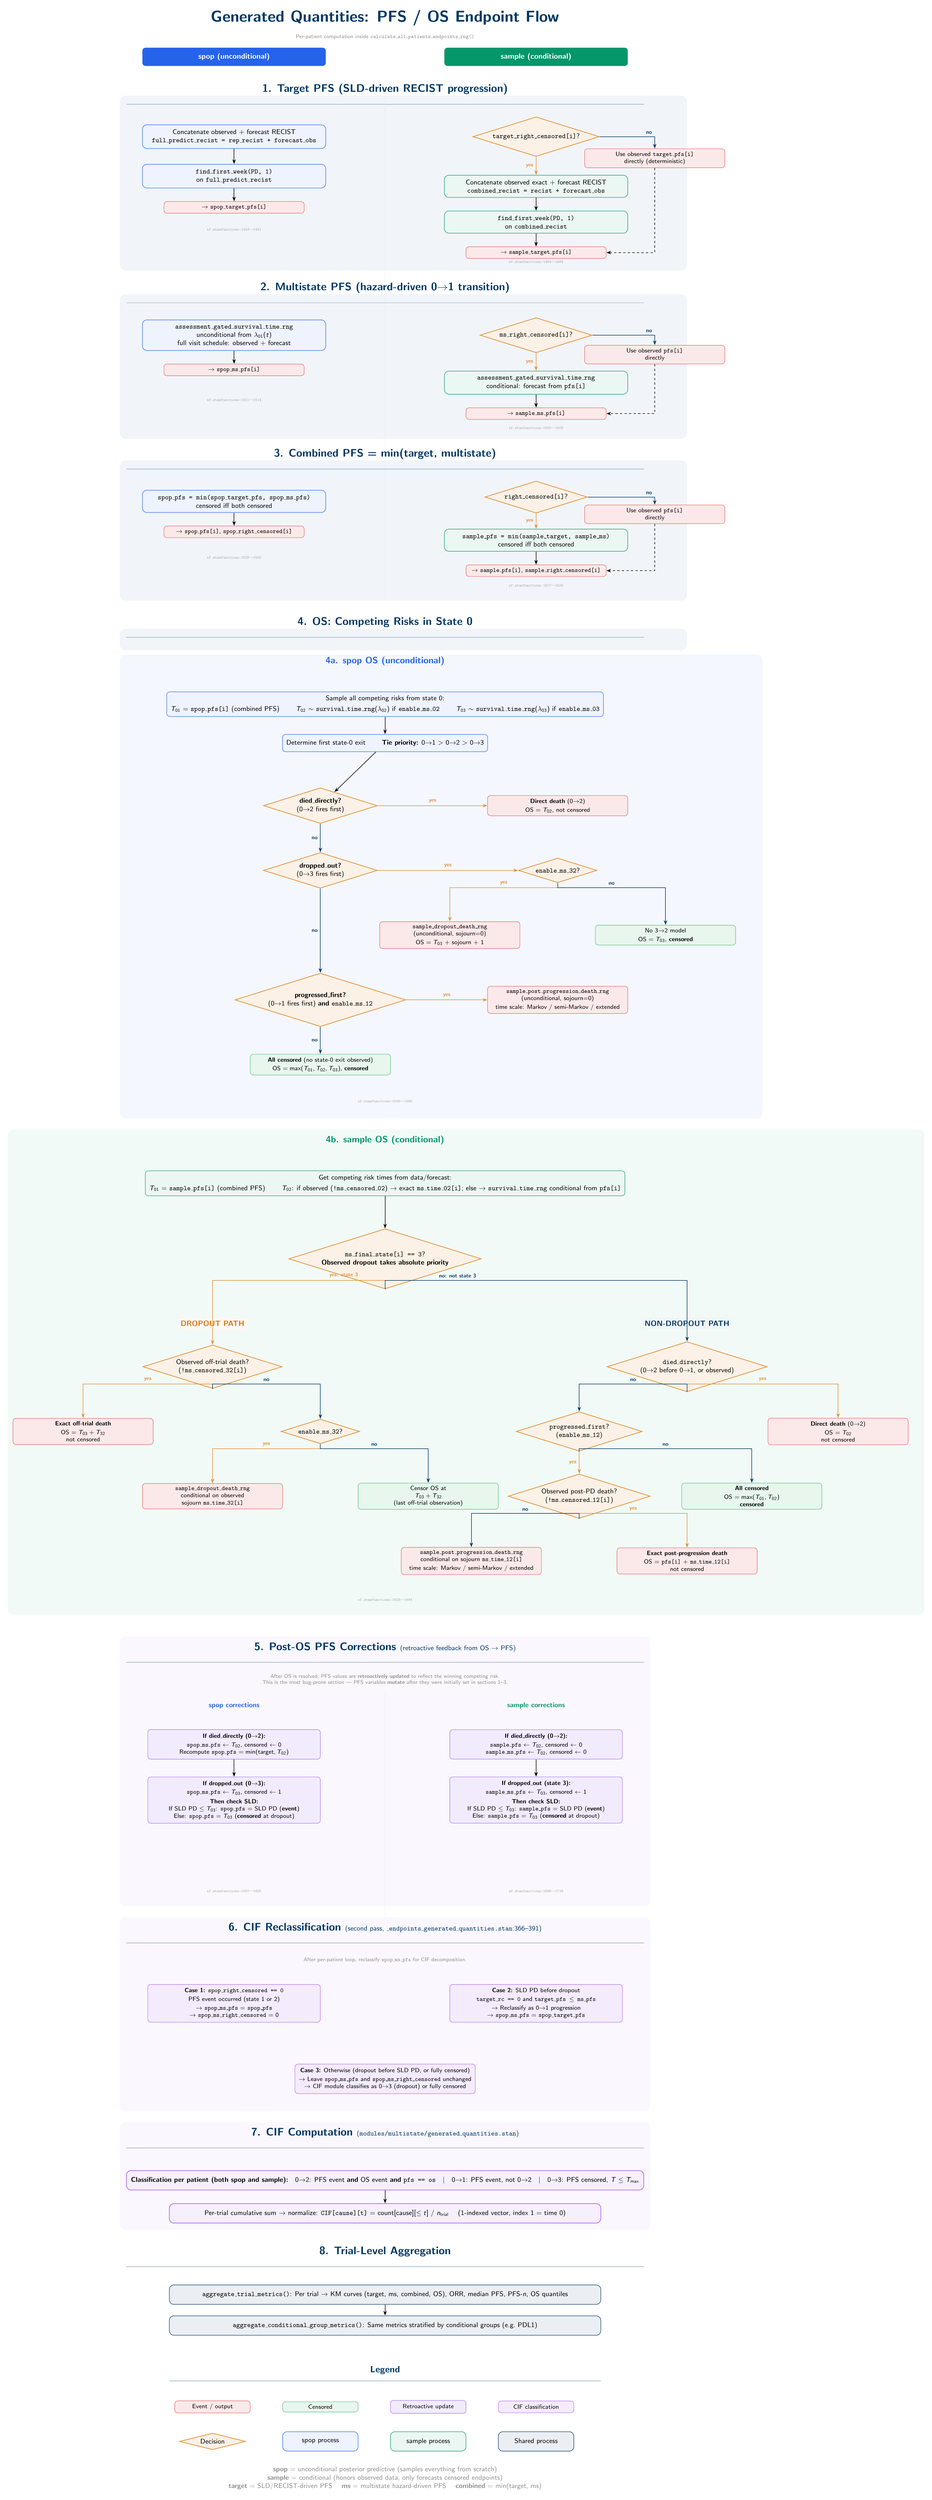
\begin{tikzpicture}[
  % --- Node styles (6.5cm wide for tree nodes) ---
  box/.style={rectangle, rounded corners=6pt, draw=#1!70, line width=0.9pt,
    fill=#1!8, minimum width=8.5cm, minimum height=0.9cm,
    text centered, align=center, inner sep=6pt, font=\small},
  box/.default=navy,
  % Wide box spanning full width
  wbox/.style={rectangle, rounded corners=6pt, draw=#1!70, line width=0.9pt,
    fill=#1!8, minimum width=20cm, minimum height=0.9cm,
    text centered, align=center, inner sep=6pt, font=\small},
  wbox/.default=navy,
  % Tree node (narrower for decision trees)
  tbox/.style={rectangle, rounded corners=4pt, draw=#1!70, line width=0.8pt,
    fill=#1!8, minimum width=8cm, minimum height=0.8cm,
    text centered, align=center, inner sep=5pt, font=\small},
  tbox/.default=navy,
  % Decision diamond
  dec/.style={diamond, draw=deccol!80, line width=0.9pt, fill=deccol!10,
    text centered, align=center, inner sep=3pt, aspect=3.2, font=\small},
  % Event result (6.5cm wide)
  ev/.style={rectangle, rounded corners=4pt, draw=eventcol!60, line width=0.7pt,
    fill=eventcol!10, minimum width=6.5cm, text centered, align=center,
    inner sep=4pt, font=\footnotesize},
  % Censored result
  cen/.style={rectangle, rounded corners=4pt, draw=censcol!60, line width=0.7pt,
    fill=censcol!10, minimum width=6.5cm, text centered, align=center,
    inner sep=4pt, font=\footnotesize},
  % Retroactive update
  upd/.style={rectangle, rounded corners=4pt, draw=updatecol!60, line width=0.7pt,
    fill=updatecol!10, minimum width=8cm, text centered, align=center,
    inner sep=5pt, font=\footnotesize},
  % CIF
  cif/.style={rectangle, rounded corners=4pt, draw=cifcol!60, line width=0.7pt,
    fill=cifcol!10, minimum width=8cm, text centered, align=center,
    inner sep=5pt, font=\footnotesize},
  % --- Arrow styles ---
  arr/.style={-Stealth, line width=0.7pt},
  darr/.style={-Stealth, line width=0.7pt, dashed},
  yarr/.style={-Stealth, line width=0.7pt, deccol!80},
  narr/.style={-Stealth, line width=0.7pt, navy},
  % --- Label styles ---
  Y/.style={font=\scriptsize\bfseries, text=deccol!80},
  N/.style={font=\scriptsize\bfseries, text=navy},
  sechead/.style={font=\Large\bfseries, text=navy},
  subsechead/.style={font=\large\bfseries, text=#1},
  subsechead/.default=navy,
  colhead/.style={font=\normalsize\bfseries, text=white, rounded corners=4pt,
    inner sep=7pt, minimum width=8.5cm, minimum height=0.8cm},
  code/.style={font=\tiny\ttfamily, text=black!35},
  note/.style={font=\scriptsize, text=black!45, align=center},
]

% Column positions for sections 1-3 and 5+
\def\spopx{-7}
\def\sampx{7}

% =====================================================================
% TITLE
% =====================================================================
\node[sechead, font=\huge\bfseries] (title) at (0, 0)
  {Generated Quantities: PFS / OS Endpoint Flow};
\node[note, below=0.15cm of title]
  {Per-patient computation inside \texttt{calculate\_all\_patients\_endpoints\_rng()}};

% =====================================================================
% COLUMN HEADERS
% =====================================================================
\node[colhead, fill=spopcol] at (\spopx, -1.8) {\textsf{spop} (unconditional)};
\node[colhead, fill=sampcol] at (\sampx, -1.8) {\textsf{sample} (conditional)};

% =====================================================================
% SECTION 1: TARGET PFS
% =====================================================================
\node[sechead] at (0, -3.3) {1. Target PFS (SLD-driven RECIST progression)};
\draw[navy!30, line width=1pt] (-12, -4.0) -- (12, -4.0);

% --- spop ---
\node[box=spopcol] (sp_tpfs) at (\spopx, -5.5)
  {Concatenate observed + forecast RECIST\\
   \texttt{full\_predict\_recist = rep\_recist + forecast\_obs}};
\node[box=spopcol, below=0.7cm of sp_tpfs] (sp_tpfs_find)
  {\texttt{find\_first\_week(PD, 1)}\\
   on \texttt{full\_predict\_recist}};
\node[ev, below=0.6cm of sp_tpfs_find] (sp_tpfs_out)
  {$\to$ \texttt{spop\_target\_pfs[i]}};
\draw[arr] (sp_tpfs) -- (sp_tpfs_find);
\draw[arr] (sp_tpfs_find) -- (sp_tpfs_out);

% --- sample ---
\node[dec] (sa_tpfs_dec) at (\sampx, -5.5)
  {\texttt{target\_right\_censored[i]}?};
\node[box=sampcol] (sa_tpfs_yes) at (\sampx, -7.8)
  {Concatenate observed exact + forecast RECIST\\
   \texttt{combined\_recist = recist + forecast\_obs}};
\node[box=sampcol, below=0.6cm of sa_tpfs_yes] (sa_tpfs_find)
  {\texttt{find\_first\_week(PD, 1)}\\
   on \texttt{combined\_recist}};
\node[ev] (sa_tpfs_no) at (12.5, -6.5)
  {Use observed \texttt{target\_pfs[i]}\\directly (deterministic)};
\node[ev, below=0.6cm of sa_tpfs_find] (sa_tpfs_out)
  {$\to$ \texttt{sample\_target\_pfs[i]}};

\draw[yarr] (sa_tpfs_dec) -- node[Y, left] {yes} (sa_tpfs_yes);
\draw[narr] (sa_tpfs_dec) -| node[N, above left] {no} (sa_tpfs_no);
\draw[arr] (sa_tpfs_yes) -- (sa_tpfs_find);
\draw[arr] (sa_tpfs_find) -- (sa_tpfs_out);
\draw[darr] (sa_tpfs_no) |- (sa_tpfs_out);

\node[code] at (\spopx, -9.8) {sf.stanfunctions:1443--1451};
\node[code] at (\sampx, -11.3) {sf.stanfunctions:1454--1484};

% Divider for sections 1-3
\draw[navy!10, line width=0.5pt] (0, -3.5) -- (0, -27);

% =====================================================================
% SECTION 2: MULTISTATE PFS
% =====================================================================
\node[sechead] at (0, -12.5) {2. Multistate PFS (hazard-driven 0$\to$1 transition)};
\draw[navy!30, line width=1pt] (-12, -13.2) -- (12, -13.2);

% --- spop ---
\node[box=spopcol] (sp_mpfs) at (\spopx, -14.7)
  {\texttt{assessment\_gated\_survival\_time\_rng}\\
   unconditional from $\lambda_{01}(t)$\\
   full visit schedule: observed + forecast};
\node[ev, below=0.6cm of sp_mpfs] (sp_mpfs_out)
  {$\to$ \texttt{spop\_ms\_pfs[i]}};
\draw[arr] (sp_mpfs) -- (sp_mpfs_out);

% --- sample ---
\node[dec] (sa_mpfs_dec) at (\sampx, -14.7)
  {\texttt{ms\_right\_censored[i]}?};
\node[box=sampcol] (sa_mpfs_yes) at (\sampx, -16.9)
  {\texttt{assessment\_gated\_survival\_time\_rng}\\
   conditional: forecast from \texttt{pfs[i]}};
\node[ev] (sa_mpfs_no) at (12.5, -15.6)
  {Use observed \texttt{pfs[i]}\\directly};
\node[ev, below=0.6cm of sa_mpfs_yes] (sa_mpfs_out)
  {$\to$ \texttt{sample\_ms\_pfs[i]}};

\draw[yarr] (sa_mpfs_dec) -- node[Y, left] {yes} (sa_mpfs_yes);
\draw[narr] (sa_mpfs_dec) -| node[N, above left] {no} (sa_mpfs_no);
\draw[arr] (sa_mpfs_yes) -- (sa_mpfs_out);
\draw[darr] (sa_mpfs_no) |- (sa_mpfs_out);

\node[code] at (\spopx, -17.7) {sf.stanfunctions:1511--1514};
\node[code] at (\sampx, -19.0) {sf.stanfunctions:1500--1509};

% =====================================================================
% SECTION 3: COMBINED PFS
% =====================================================================
\node[sechead] at (0, -20.2) {3. Combined PFS = min(target, multistate)};
\draw[navy!30, line width=1pt] (-12, -20.9) -- (12, -20.9);

% --- spop ---
\node[box=spopcol] (sp_cpfs) at (\spopx, -22.4)
  {\texttt{spop\_pfs = min(spop\_target\_pfs, spop\_ms\_pfs)}\\
   censored iff both censored};
\node[ev, below=0.6cm of sp_cpfs] (sp_cpfs_out)
  {$\to$ \texttt{spop\_pfs[i]}, \texttt{spop\_right\_censored[i]}};
\draw[arr] (sp_cpfs) -- (sp_cpfs_out);

% --- sample ---
\node[dec] (sa_cpfs_dec) at (\sampx, -22.2)
  {\texttt{right\_censored[i]}?};
\node[box=sampcol] (sa_cpfs_yes) at (\sampx, -24.2)
  {\texttt{sample\_pfs = min(sample\_target, sample\_ms)}\\
   censored iff both censored};
\node[ev] (sa_cpfs_no) at (12.5, -23.0)
  {Use observed \texttt{pfs[i]}\\directly};
\node[ev, below=0.6cm of sa_cpfs_yes] (sa_cpfs_out)
  {$\to$ \texttt{sample\_pfs[i]}, \texttt{sample\_right\_censored[i]}};

\draw[yarr] (sa_cpfs_dec) -- node[Y, left] {yes} (sa_cpfs_yes);
\draw[narr] (sa_cpfs_dec) -| node[N, above left] {no} (sa_cpfs_no);
\draw[arr] (sa_cpfs_yes) -- (sa_cpfs_out);
\draw[darr] (sa_cpfs_no) |- (sa_cpfs_out);

\node[code] at (\spopx, -25.0) {sf.stanfunctions:1528--1530};
\node[code] at (\sampx, -26.3) {sf.stanfunctions:1517--1526};

% =====================================================================
% SECTION 4: OS — COMPETING RISKS IN STATE 0
% =====================================================================
\node[sechead] at (0, -28.0) {4. OS: Competing Risks in State 0};
\draw[navy!30, line width=1pt] (-12, -28.7) -- (12, -28.7);

% ====================================================================
%   4a. SPOP OS (unconditional) — FULL WIDTH, CASCADE LAYOUT
% ====================================================================
\node[subsechead=spopcol] at (0, -29.8)
  {4a. spop OS (unconditional)};

% Input
\node[tbox=spopcol] (sp_cr) at (0, -31.8)
  {Sample all competing risks from state 0:\\[3pt]
   $T_{01}$ = \texttt{spop\_pfs[i]} (combined PFS) \qquad
   $T_{02}$ $\sim$ \texttt{survival\_time\_rng}($\lambda_{02}$) if \texttt{enable\_ms\_02} \qquad
   $T_{03}$ $\sim$ \texttt{survival\_time\_rng}($\lambda_{03}$) if \texttt{enable\_ms\_03}};

% First exit determination
\node[tbox=spopcol, below=0.8cm of sp_cr] (sp_first)
  {Determine first state-0 exit \qquad
   \textbf{Tie priority:} 0$\to$1 $>$ 0$\to$2 $>$ 0$\to$3};

\draw[arr] (sp_cr) -- (sp_first);

% === Cascade: main chain at x=-3, YES outcomes at x=8 ===

% Level 1: died_directly?
\node[dec] (sp_d_died) at (-3, -36.5)
  {\textbf{died\_directly?}\\(0$\to$2 fires first)};
\node[ev] (sp_died_out) at (8, -36.5)
  {\textbf{Direct death} (0$\to$2)\\[2pt]
   OS $= T_{02}$, not censored};

\draw[arr] (sp_first) -- (sp_d_died);
\draw[yarr] (sp_d_died) -- node[Y, above] {yes} (sp_died_out);

% Level 2: dropped_out?
\node[dec] (sp_d_drop) at (-3, -39.5)
  {\textbf{dropped\_out?}\\(0$\to$3 fires first)};

\draw[narr] (sp_d_died) -- node[N, left] {no} (sp_d_drop);

% Dropout sub-decision: enable_ms_32?
\node[dec] (sp_d_32) at (8, -39.5)
  {\texttt{enable\_ms\_32}?};

\draw[yarr] (sp_d_drop) -- node[Y, above] {yes} (sp_d_32);

\node[ev] (sp_32_yes) at (3, -42.5)
  {\texttt{sample\_dropout\_death\_rng}\\(unconditional, sojourn=0)\\[2pt]
   OS $= T_{03}$ + sojourn + 1};
\node[cen] (sp_32_no) at (13, -42.5)
  {No 3$\to$2 model\\[2pt]
   OS $= T_{03}$, \textbf{censored}};

\draw[yarr] (sp_d_32) -- ++(0,-0.8) -| (sp_32_yes)
  node[Y, pos=0.25, above] {yes};
\draw[narr] (sp_d_32) -- ++(0,-0.8) -| (sp_32_no)
  node[N, pos=0.25, above] {no};

% Level 3: progressed_first?
\node[dec] (sp_d_prog) at (-3, -45.5)
  {\textbf{progressed\_first?}\\(0$\to$1 fires first) \textbf{and} \texttt{enable\_ms\_12}};
\node[ev] (sp_prog_out) at (8, -45.5)
  {\texttt{sample\_post\_progression\_death\_rng}\\(unconditional, sojourn=0)\\[2pt]
   time scale: Markov / semi-Markov / extended};

\draw[narr] (sp_d_drop) -- node[N, left] {no} (sp_d_prog);
\draw[yarr] (sp_d_prog) -- node[Y, above] {yes} (sp_prog_out);

% Level 4: all censored
\node[cen] (sp_allcens) at (-3, -48.5)
  {\textbf{All censored} (no state-0 exit observed)\\[2pt]
   OS $= \max(T_{01}, T_{02}, T_{03})$, \textbf{censored}};

\draw[narr] (sp_d_prog) -- node[N, left] {no} (sp_allcens);

\node[code] at (0, -50.2) {sf.stanfunctions:1536--1595};

% ====================================================================
%   4b. SAMPLE OS (conditional) — FULL WIDTH, CASCADE LAYOUT
% ====================================================================
\node[subsechead=sampcol] at (0, -52.0)
  {4b. sample OS (conditional)};

% Input
\node[tbox=sampcol] (sa_cr) at (0, -54.0)
  {Get competing risk times from data/forecast:\\[3pt]
   $T_{01}$ = \texttt{sample\_pfs[i]} (combined PFS) \qquad
   $T_{02}$: if observed (\texttt{!ms\_censored\_02}) $\to$ exact \texttt{ms\_time\_02[i]};
   else $\to$ \texttt{survival\_time\_rng} conditional from \texttt{pfs[i]}};

% Top decision: dropout?
\node[dec] (sa_d_drop) at (0, -57.5)
  {\texttt{ms\_final\_state[i] == 3}?\\
   \textbf{Observed dropout takes absolute priority}};

\draw[arr] (sa_cr) -- (sa_d_drop);

% ===== DROPOUT PATH (left sub-tree) =====
\node[font=\normalsize\bfseries, text=deccol, fill=deccol!5, rounded corners=3pt, inner sep=4pt]
  at (-8, -60.5) {DROPOUT PATH};

\node[dec] (sa_dd_obs32) at (-8, -62.5)
  {Observed off-trial death?\\(\texttt{!ms\_censored\_32[i]})};

\draw[yarr] (sa_d_drop) -- ++(0,-1.0) -| (sa_dd_obs32)
  node[Y, pos=0.12, above] {yes: state 3};

% Observed 3->2: exact
\node[ev] (sa_dd_exact) at (-14, -65.5)
  {\textbf{Exact off-trial death}\\[2pt]
   OS $= T_{03} + T_{32}$\\
   not censored};

\draw[yarr] (sa_dd_obs32) -- ++(0,-0.8) -| (sa_dd_exact)
  node[Y, pos=0.25, above] {yes};

% Not observed: enable_ms_32?
\node[dec] (sa_dd_en32) at (-3, -65.5)
  {\texttt{enable\_ms\_32}?};

\draw[narr] (sa_dd_obs32) -- ++(0,-0.8) -| (sa_dd_en32)
  node[N, pos=0.25, above] {no};

% enable=yes: forecast
\node[ev] (sa_dd_fore) at (-8, -68.5)
  {\texttt{sample\_dropout\_death\_rng}\\conditional on observed\\sojourn \texttt{ms\_time\_32[i]}};

\draw[yarr] (sa_dd_en32) -- ++(0,-0.8) -| (sa_dd_fore)
  node[Y, pos=0.25, above] {yes};

% enable=no: censor
\node[cen] (sa_dd_cens) at (2, -68.5)
  {Censor OS at\\$T_{03} + T_{32}$\\(last off-trial observation)};

\draw[narr] (sa_dd_en32) -- ++(0,-0.8) -| (sa_dd_cens)
  node[N, pos=0.25, above] {no};

% ===== NON-DROPOUT PATH (right sub-tree) =====
\node[font=\normalsize\bfseries, text=navy, fill=navy!5, rounded corners=3pt, inner sep=4pt]
  at (14, -60.5) {NON-DROPOUT PATH};

\node[dec] (sa_nd_died) at (14, -62.5)
  {\texttt{died\_directly}?\\(0$\to$2 before 0$\to$1, or observed)};

\draw[narr] (sa_d_drop) -- ++(0,-1.0) -| (sa_nd_died)
  node[N, pos=0.12, above] {no: not state 3};

% Died directly: exact
\node[ev] (sa_nd_died_out) at (21, -65.5)
  {\textbf{Direct death} (0$\to$2)\\[2pt]
   OS $= T_{02}$\\
   not censored};

\draw[yarr] (sa_nd_died) -- ++(0,-0.8) -| (sa_nd_died_out)
  node[Y, pos=0.25, above] {yes};

% Not died: progressed?
\node[dec] (sa_nd_prog) at (9, -65.5)
  {\texttt{progressed\_first}?\\(\texttt{enable\_ms\_12})};

\draw[narr] (sa_nd_died) -- ++(0,-0.8) -| (sa_nd_prog)
  node[N, pos=0.25, above] {no};

% Progressed YES: observed 1->2?
\node[dec] (sa_nd_obs12) at (9, -68.5)
  {Observed post-PD death?\\(\texttt{!ms\_censored\_12[i]})};

\draw[yarr] (sa_nd_prog) -- (sa_nd_obs12)
  node[Y, pos=0.5, left] {yes};

% Not progressed: all censored
\node[cen] (sa_nd_allcens) at (17, -68.5)
  {\textbf{All censored}\\[2pt]
   OS $= \max(T_{01}, T_{02})$\\
   \textbf{censored}};

\draw[narr] (sa_nd_prog) -- ++(0,-0.8) -| (sa_nd_allcens)
  node[N, pos=0.25, above] {no};

% Observed 1->2: exact
\node[ev] (sa_nd_12_exact) at (14, -71.5)
  {\textbf{Exact post-progression death}\\[2pt]
   OS $=$ \texttt{pfs[i]} $+$ \texttt{ms\_time\_12[i]}\\
   not censored};

\draw[yarr] (sa_nd_obs12) -- ++(0,-0.8) -| (sa_nd_12_exact)
  node[Y, pos=0.25, above] {yes};

% Censored 1->2: forecast
\node[ev] (sa_nd_12_fore) at (4, -71.5)
  {\texttt{sample\_post\_progression\_death\_rng}\\conditional on sojourn \texttt{ms\_time\_12[i]}\\[2pt]
   time scale: Markov / semi-Markov / extended};

\draw[narr] (sa_nd_obs12) -- ++(0,-0.8) -| (sa_nd_12_fore)
  node[N, pos=0.25, above] {no};

\node[code] at (0, -73.3) {sf.stanfunctions:1623--1694};

% =====================================================================
% SECTION 5: POST-OS PFS CORRECTIONS
% =====================================================================
\node[sechead] at (0, -75.5) {5. Post-OS PFS Corrections \textnormal{\small(retroactive feedback from OS $\to$ PFS)}};
\draw[navy!30, line width=1pt] (-12, -76.2) -- (12, -76.2);

\node[note] at (0, -77.0)
  {After OS is resolved, PFS values are \textbf{retroactively updated} to reflect the winning competing risk.\\
   This is the most bug-prone section --- PFS variables \textbf{mutate} after they were initially set in sections 1--3.};

% Divider for sections 5+
\draw[navy!10, line width=0.5pt] (0, -77.5) -- (0, -88);

% --- spop corrections ---
\node[subsechead=spopcol, font=\small\bfseries] at (\spopx, -78.2) {spop corrections};

\node[upd] (sp_upd_died) at (\spopx, -80.0)
  {\textbf{If died\_directly (0$\to$2):}\\[2pt]
   \texttt{spop\_ms\_pfs} $\leftarrow T_{02}$, censored $\leftarrow$ 0\\
   Recompute \texttt{spop\_pfs} $= \min(\text{target}, T_{02})$};

\node[upd, below=0.8cm of sp_upd_died] (sp_upd_drop)
  {\textbf{If dropped\_out (0$\to$3):}\\[2pt]
   \texttt{spop\_ms\_pfs} $\leftarrow T_{03}$, censored $\leftarrow$ 1\\[3pt]
   \textbf{Then check SLD:}\\
   If SLD PD $\leq T_{03}$: \texttt{spop\_pfs} $=$ SLD PD (\textbf{event})\\
   Else: \texttt{spop\_pfs} $= T_{03}$ (\textbf{censored} at dropout)};

\draw[arr] (sp_upd_died) -- (sp_upd_drop);

% --- sample corrections ---
\node[subsechead=sampcol, font=\small\bfseries] at (\sampx, -78.2) {sample corrections};

\node[upd] (sa_upd_died) at (\sampx, -80.0)
  {\textbf{If died\_directly (0$\to$2):}\\[2pt]
   \texttt{sample\_pfs} $\leftarrow T_{02}$, censored $\leftarrow$ 0\\
   \texttt{sample\_ms\_pfs} $\leftarrow T_{02}$, censored $\leftarrow$ 0};

\node[upd, below=0.8cm of sa_upd_died] (sa_upd_drop)
  {\textbf{If dropped\_out (state 3):}\\[2pt]
   \texttt{sample\_ms\_pfs} $\leftarrow T_{03}$, censored $\leftarrow$ 1\\[3pt]
   \textbf{Then check SLD:}\\
   If SLD PD $\leq T_{03}$: \texttt{sample\_pfs} $=$ SLD PD (\textbf{event})\\
   Else: \texttt{sample\_pfs} $= T_{03}$ (\textbf{censored} at dropout)};

\draw[arr] (sa_upd_died) -- (sa_upd_drop);

\node[code] at (\spopx, -86.8) {sf.stanfunctions:1597--1620};
\node[code] at (\sampx, -86.8) {sf.stanfunctions:1696--1719};

% =====================================================================
% SECTION 6: CIF RECLASSIFICATION
% =====================================================================
\node[sechead] at (0, -88.5)
  {6. CIF Reclassification \textnormal{\small(second pass, \texttt{\_endpoints\_generated\_quantities.stan}:366--391)}};
\draw[navy!30, line width=1pt] (-12, -89.2) -- (12, -89.2);

\node[note] at (0, -90.0)
  {After per-patient loop, reclassify \texttt{spop\_ms\_pfs} for CIF decomposition.};

\node[cif] (cif1) at (-7, -92.0)
  {\textbf{Case 1:} \texttt{spop\_right\_censored == 0}\\[2pt]
   PFS event occurred (state 1 or 2)\\[2pt]
   $\to$ \texttt{spop\_ms\_pfs} $=$ \texttt{spop\_pfs}\\
   $\to$ \texttt{spop\_ms\_right\_censored} $=$ 0};

\node[cif] (cif2) at (7, -92.0)
  {\textbf{Case 2:} SLD PD before dropout\\[2pt]
   \texttt{target\_rc == 0} and \texttt{target\_pfs $\leq$ ms\_pfs}\\[2pt]
   $\to$ Reclassify as 0$\to$1 progression\\
   $\to$ \texttt{spop\_ms\_pfs} $=$ \texttt{spop\_target\_pfs}};

\node[cif] (cif3) at (0, -95.5)
  {\textbf{Case 3:} Otherwise (dropout before SLD PD, or fully censored)\\[2pt]
   $\to$ Leave \texttt{spop\_ms\_pfs} and \texttt{spop\_ms\_right\_censored} unchanged\\
   $\to$ CIF module classifies as 0$\to$3 (dropout) or fully censored};

% =====================================================================
% SECTION 7: CIF COMPUTATION
% =====================================================================
\node[sechead] at (0, -98.0)
  {7. CIF Computation \textnormal{\small(\texttt{modules/multistate/generated\_quantities.stan})}};
\draw[navy!30, line width=1pt] (-12, -98.7) -- (12, -98.7);

\node[wbox=cifcol] (cif_class) at (0, -100.2)
  {\textbf{Classification per patient (both spop and sample):}\quad
   0$\to$2: PFS event \textbf{and} OS event \textbf{and} \texttt{pfs == os}\quad$|$\quad
   0$\to$1: PFS event, not 0$\to$2\quad$|$\quad
   0$\to$3: PFS censored, $T \leq T_{\max}$};

\node[wbox=cifcol, below=0.6cm of cif_class] (cif_cum)
  {Per-trial cumulative sum $\to$ normalize:
   \texttt{CIF[cause][t]} $=$ count[cause][$\leq t$] / $n_{\text{trial}}$
   \quad (1-indexed vector, index 1 = time 0)};

\draw[arr] (cif_class) -- (cif_cum);

% =====================================================================
% SECTION 8: TRIAL AGGREGATION
% =====================================================================
\node[sechead] at (0, -103.5)
  {8. Trial-Level Aggregation};
\draw[navy!30, line width=1pt] (-12, -104.2) -- (12, -104.2);

\node[wbox] (agg) at (0, -105.5)
  {\texttt{aggregate\_trial\_metrics()}: Per trial $\to$ KM curves (target, ms, combined, OS),
   ORR, median PFS, PFS-$n$, OS quantiles};

\node[wbox, below=0.5cm of agg] (cond_agg)
  {\texttt{aggregate\_conditional\_group\_metrics()}: Same metrics stratified by conditional groups (e.g.\ PDL1)};

\draw[arr] (agg) -- (cond_agg);

% =====================================================================
% LEGEND
% =====================================================================
\node[font=\large\bfseries, text=navy] at (0, -109.0) {Legend};
\draw[navy!30, line width=1pt] (-10, -109.5) -- (10, -109.5);

\node[ev, minimum width=3.5cm] at (-8, -110.7) {Event / output};
\node[cen, minimum width=3.5cm] at (-3, -110.7) {Censored};
\node[upd, minimum width=3.5cm] at (2, -110.7) {Retroactive update};
\node[cif, minimum width=3.5cm] at (7, -110.7) {CIF classification};

\node[dec, minimum width=3cm, aspect=4] at (-8, -112.3) {Decision};
\node[box=spopcol, minimum width=3.5cm] at (-3, -112.3) {spop process};
\node[box=sampcol, minimum width=3.5cm] at (2, -112.3) {sample process};
\node[box=navy, minimum width=3.5cm] at (7, -112.3) {Shared process};

\node[note, font=\small] at (0, -114.0)
  {\textbf{spop} = unconditional posterior predictive (samples everything from scratch)\\
   \textbf{sample} = conditional (honors observed data, only forecasts censored endpoints)\\
   \textbf{target} = SLD/RECIST-driven PFS \quad
   \textbf{ms} = multistate hazard-driven PFS \quad
   \textbf{combined} = min(target, ms)};

% =====================================================================
% BACKGROUND SECTIONS
% =====================================================================
\begin{scope}[on background layer]
  % Sections 1-3
  \fill[secbg, rounded corners=8pt] (-12.3, -3.6) rectangle (14, -11.7);
  \fill[secbg, rounded corners=8pt] (-12.3, -12.8) rectangle (14, -19.5);
  \fill[secbg, rounded corners=8pt] (-12.3, -20.5) rectangle (14, -27.0);
  % Section 4 header
  \fill[secbg, rounded corners=8pt] (-12.3, -28.3) rectangle (14, -29.3);
  % Section 4a (spop OS)
  \fill[spopcol!5, rounded corners=8pt] (-12.3, -29.5) rectangle (17.5, -51.0);
  % Section 4b (sample OS)
  \fill[sampcol!5, rounded corners=8pt] (-17.5, -51.5) rectangle (25, -74.0);
  % Section 5
  \fill[updatecol!4, rounded corners=8pt] (-12.3, -75.0) rectangle (12.3, -87.5);
  % Section 6
  \fill[cifcol!4, rounded corners=8pt] (-12.3, -88.0) rectangle (12.3, -97.0);
  % Section 7
  \fill[cifcol!4, rounded corners=8pt] (-12.3, -97.5) rectangle (12.3, -102.5);
\end{scope}

\end{tikzpicture}

\end{document}
